\chapter{XML and APIIS model}

Writing a model file as a simple text file always consumes a lot of
time and is not protected of making mistakes that can have effect
on further work with other APIIS tools. Working with a text editor
usual does not give the completely picture of a document stricture
that makes changes in the model file difficult and slow. In order
to use faster and safety way for writing and editing a model file
XML standard is implemented for describing data model structure of
APIIS. 


\section{Why XML?}

:) 


\section{Needed modules}

The names of needed modules are written in file \emph{needed\_modules}
in pdbl tree. 


\subsection{Parsing XML document}

From many existing perl parsers of XML documents are chosen two that
are standard for Perl 5.6.1 - XML::Parser and XML::Writer. Usual these
modules are installed during regular perl installation in folder named
\emph{xml}. They use stream methods of parsing that are faster and
take less memory for storage of data elements which was the reason
for their usage.

For better XML print a code, version of XML::Writer, \emph{myWriter}
is improved specially for APIIS.


\subsection{Document Type Definition (DTD) of APIIS model in XML standard }

APIIS model file is described in XML DTD format via the structure
given in the figure \ref{modeldtd} . The root element is the \emph{model}
with sub elements or children \emph{general} and \emph{table}. The
sub elements of \emph{table} are \emph{column} and \emph{TABLE. TRIGGER}
and \emph{CONSTRAINTS} are sub elements of \emph{TABLE.}

%
\begin{figure}[htbp]

\caption{The XML structure of APIIS model \label{modeldtd}}

\begin{center}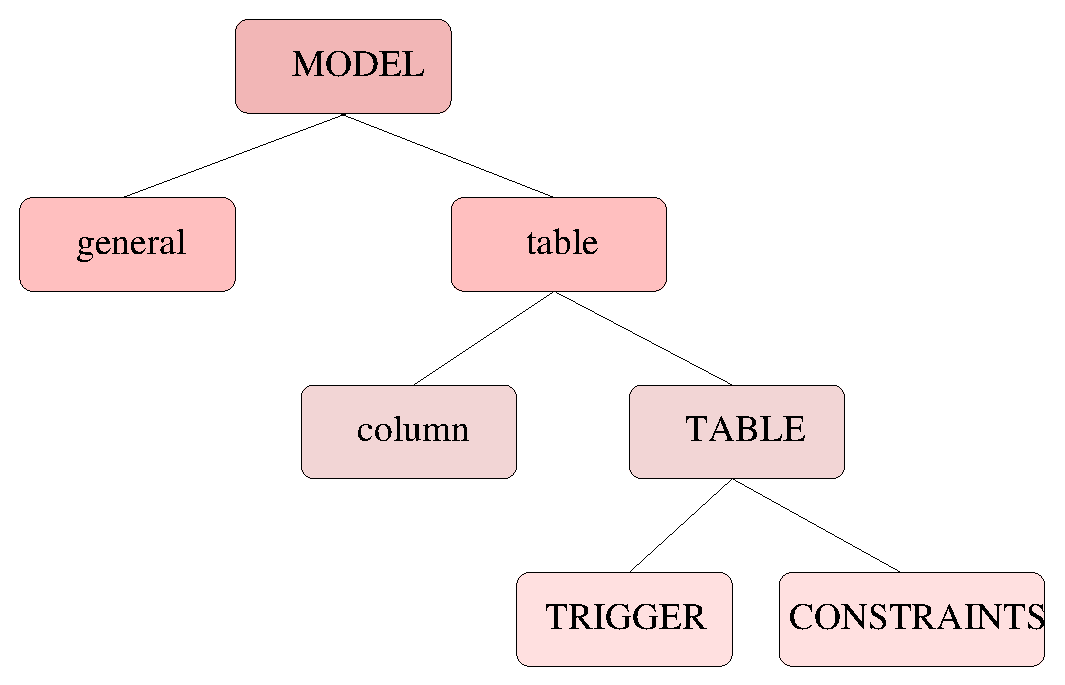
\includegraphics[%
  scale=0.4]{./XML-model/modeldtd.eps}\end{center}
\end{figure}


The DTD file on the figure \ref{DTDfile} shows the elements definitions
in APIIS model XML format as well as their attributes' lists. As attributes
are better processed by some XML editors they are preferred here.
Usage of attributes allows default values that facilitates the inserts
of model elements. It can be seen that elements marked by '+' are
these appearing more than ones in the model structure like \emph{table}
and \emph{column}.

%
\begin{table}[htbp]

\caption{DTD file of APIIS model \label{DTDfile}}

{\scriptsize <!DOCTYPE model {[}}{\scriptsize \par}

{\scriptsize <!ELEMENT model (general,table+)>}{\scriptsize \par}

{\scriptsize <!ELEMENT general EMPTY>}{\scriptsize \par}

{\scriptsize <!ATTLIST general }{\scriptsize \par}

{\scriptsize dbdriver (Pg|Oracle|CSV|InterBase|Sybase) \char`\"{}Pg\char`\"{}}{\scriptsize \par}

{\scriptsize dbname CDATA \#REQUIRED}{\scriptsize \par}

{\scriptsize dbhost CDATA \char`\"{}localhost\char`\"{}}{\scriptsize \par}

{\scriptsize dbport CDATA \char`\"{}5432\char`\"{}}{\scriptsize \par}

{\scriptsize dbuser CDATA \char`\"{}\$user\char`\"{}}{\scriptsize \par}

{\scriptsize dbpassword CDATA \char`\"{}\char`\"{}>}{\scriptsize \par}

{\scriptsize <!ELEMENT table (column+,TABLE)>}{\scriptsize \par}

{\scriptsize <!ATTLIST table}{\scriptsize \par}

{\scriptsize name CDATA \#REQUIRED>}{\scriptsize \par}

{\scriptsize <!ELEMENT column EMPTY>}{\scriptsize \par}

{\scriptsize <!ATTLIST column DATA CDATA \char`\"{}\char`\"{}}{\scriptsize \par}

{\scriptsize name CDATA \#REQUIRED}{\scriptsize \par}

{\scriptsize DATATYPE}{\scriptsize \par}

{\scriptsize (CHAR|HUGEINT|BIGINT|SMALLINT|DATE|TIME|TIMESTAMP|SMALLFLOAT|BIGFLOAT|BOOL)
\char`\"{}CHAR\char`\"{}}{\scriptsize \par}

{\scriptsize LENGTH CDATA \char`\"{}20\char`\"{}}{\scriptsize \par}

{\scriptsize DESCRIPTION CDATA \#REQUIRED}{\scriptsize \par}

{\scriptsize DEFAULT CDATA \char`\"{}\char`\"{}}{\scriptsize \par}

{\scriptsize CHECK CDATA \char`\"{}\char`\"{}}{\scriptsize \par}

{\scriptsize MODIFY CDATA \char`\"{}\char`\"{}}{\scriptsize \par}

{\scriptsize ERROR CDATA \char`\"{}\char`\"{}>}{\scriptsize \par}

{\scriptsize <!ELEMENT TABLE (TRIGGER,CONSTRAINTS)> }{\scriptsize \par}

{\scriptsize <!ELEMENT TRIGGER EMPTY>}{\scriptsize \par}

{\scriptsize <!ATTLIST TRIGGER PREINSERT CDATA \char`\"{}\char`\"{}}{\scriptsize \par}

{\scriptsize POSTINSERT CDATA \char`\"{}\char`\"{}}{\scriptsize \par}

{\scriptsize PREUPDATE CDATA \char`\"{}\char`\"{}}{\scriptsize \par}

{\scriptsize POSTUPDATE CDATA \char`\"{}\char`\"{}}{\scriptsize \par}

{\scriptsize PREDELETE CDATA \char`\"{}\char`\"{}}{\scriptsize \par}

{\scriptsize POSTDELETE CDATA \char`\"{}\char`\"{}>}{\scriptsize \par}

{\scriptsize <!ELEMENT CONSTRAINTS EMPTY>}{\scriptsize \par}

{\scriptsize <!ATTLIST CONSTRAINTS }{\scriptsize \par}

{\scriptsize PRIMARYKEY CDATA \char`\"{}\char`\"{}}{\scriptsize \par}

{\scriptsize SEQUENCE CDATA \char`\"{}\char`\"{}}{\scriptsize \par}

{\scriptsize INDEX CDATA \char`\"{}\char`\"{}> {]}>}
\end{table}



\subsection{Converting the model file to XML format}

The perl code \emph{model2xml.pl} converts the model file to XML format.
Location is in \emph{pdbl/bin}. The syntax is the next:

\emph{model2xml model\_filename xml\_filename,} where the first argument
is the model file name and second is the xml file name that is better
to have extension \emph{xml} for further work with some XML editors. 


\subsection{Extracting APIIS model file from XML document }

Extracting the mode file from xml formatted file is done by perl code
\emph{xml2model}.\emph{pl} located in \emph{pdbl/bin}. The syntax
is the next:

\emph{xml2model} \emph{xml\_filename model\_filename}, where the arguments
are with the same meaning as in 8.2.3. Here the default values of
the elements' arguments are taken automatically from DTD file. The
size of xml format file is twice less than usual model format file
because all default values are not saved.


\subsection{Editing of XML documents }

XML editors process XML documents usual in GUI environment where all
existing xml elements are accessible for editing, moving and copies.
All operations are controlled via DTD file or XML scheme. The entire
structure of the document is in tree view that can be easy processed. 

So far editor of choice is \emph{Xerlin} available in http://www.xerlin.org.
It demands Java machine to be installed. 


\section{How to use? }

The idea is using the document type definition in 'model.dtd' and
working with the program 'xerlin' to write the model file in format
of xml document. The process is facilitated via usage of libraries
of elements: columns and tables in which the main DB structure of
APIIS is implemented. 


\subsection{Creating a new model file}

Steps:

\begin{enumerate}
\item Open library apiis.xmllib from where the necessary elements could
be copied or simply 'drop and drag'.
\item Start new file with choice of DTD file model.dtd from pdbl/lib that
will be used for xml structure control and checks.
\item Insert the root element of the document - \emph{model} and first its
child - general. 
\item Take from library the main table xml equivalents
\item Insert other elements
\end{enumerate}
For creating a complete model file is recommended to start with root
element although the program offers you to choose from which element
to start.

All attributes with mandatory values (\#REQUIERED) are marked to be
inserted before next element starts. The context menus of the right
mouse button in Xerlin offer to choose among legal operations and
elements according the DTD and current content of the document. All
operations are restricted by context and logical structure in DTD
that protect the user from making mistakes. In the context menu only
legal elements are accessed and can be inserted after, before or into
a current element.

When an element is chosen its attributes are shown in right panel,
default values are there and we insert only attribute values which
are different from default ones.

The result file contains all elements of table and column types and
their attributes. The default attributes' values are not recorded
in this file if the property 'merlot.write.default-attr' has a value
'false' in preference panel. 


\subsection{Editing the model file}

To produce APIIS format model file in syntax we use in APIIS environment
is used the module \emph{xml2model.pl}. The result file is used by
other APIIS applications. In case the model file needs to be changed
in Xerlin it is reversed in xml format via module model2xml.pl. 


\subsection{Using alternative XML editors.}

In case Xerlin is not accessible another xml editor could be used. 

\begin{enumerate}
\item xemacs 
\item kate
\item kxmleditor
\end{enumerate}
If they are appropriate will be investigated.(so far they are weaker
than Xerlin) 


